\chapter{Current Development}\label{C:eda}
As detailed in the project proposal, the first weeks of project development have focused on an initial EDA. While taking longer than expected, this was completed in its entirety, with several stages of analysis focusing on data cleaning (\Cref{S:IDC}), examining feature distributions (\Cref{SS:distributions} \& \Cref{fig:boxplots}),  trends in feature distribution (\Cref{SS:temporal_trends} \& \Cref{SS:spatial_analysis}), and inter-variable correlations (\Cref{SS:correlation_analysis}). 

Initial analysis was performed without preprocessing to understand the nature of the initial dataset. This analysis excludes the positional constants \texttt{x\_coordinate} and \texttt{y\_coordinate}, as well as the inferred variable \texttt{year}, as these are used for reference and not for prediction or evaluation. 

\section{Initial Data Cleaning}\label{S:IDC}

Some minor data cleaning was performed before analysis, so as not to skew the results. Most prominently, several values in the dataset were found to be filler values or \texttt{NaN} values \textit{(Not a Number - used to represent empty or faulty data points)}. This can be seen in \Cref{table:nan_counts}.

\begin{table}[H]
  \centering
  \begin{tabular}{|l|r|r|}
  \hline
  Measure & Count & Proportion of Measure \\ \hline
  ice\_velocity & 146,083 & 65.30\% \\ \hline
  ice\_thickness & 143,819 & 64.29\% \\ \hline
  ocean\_temperature & 29,584 & 13.22\% \\ \hline
  precipitation & 385 & \textless{0.01}\% \\ \hline
  ice\_mask & 124 & \textless{0.01}\% \\ \hline
  \end{tabular}
  \caption{Counts of \texttt{NaN} and Filler Values in Dataset}
  \label{table:nan_counts}
\end{table}
  
The large proportion of \texttt{NaN} and filler values in the dataset are due to the relationship between ocean and ice cells. The majority of cells are in the ocean surrounding the ice sheet –- and thus often do not have ice measurements. This causes the ice measurements \textit{(ice\_thickness, ice\_velocity, ice\_mask)} to contain \texttt{NaN} or filler values within these cells \textit{(typically 0)}. Inversely, the ocean temperature measurements are \texttt{NaN} or filler values in cells containing ice \textit{(typically 9.969...e+36)}, though this value is also used for cells without any measurement taken.

For ocean temperature values, the datapoints containing \texttt{NaN} or filler values were removed from the dataset. This was done as these values are found exclusively around the perimeter of the collected data, and only used to  provide a square grid despite the circular nature of the collected data. This can be viewed with a spatial heatmap \textit{(See \Cref{fig:spatial_heatmap_air_temp})} of the air temperature values, which shows a clear circular border around the data where these values are not present.

\begin{figure}[ht]
  \centering
  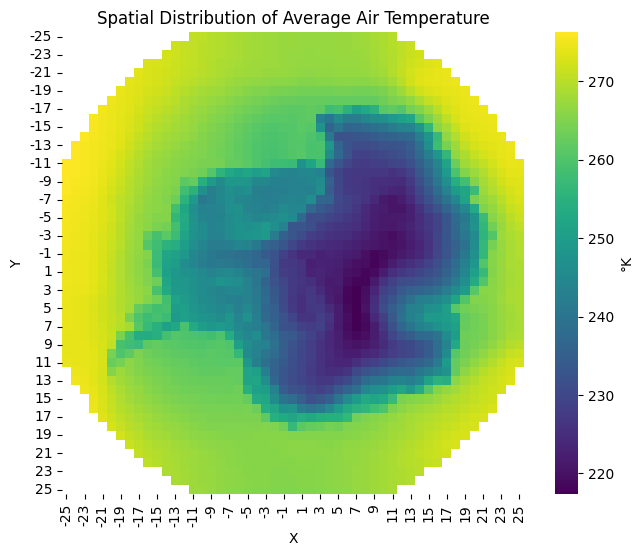
\includegraphics[width=0.65\textwidth]{images/air_temperature/air_temperature_spatial_heatmap.png}
  \caption{Spatial Heatmap of Average Air Temperature Values (°K)}
  \label{fig:spatial_heatmap_air_temp}
\end{figure}

All filler values for the \texttt{ice\_mask} variable were set to 4, as this value is used to represent open ocean. Additionally, all measures were quantised into integers to reflect the discrete nature of the variable, and to discard some minor variations currently found in the value. The values for ice velocity and ice thickness do not have set values for ocean cells, so these were left as \texttt{NaN} values for the initial analysis. Finally, the few \texttt{NaN} values in the precipitation variable were filled with the mean of the variable, as these appeared randomly distributed throughout the dataset.

\section{Univariate Analysis}\label{S:UVA}

The initial data cleaning allowed univariate analysis to be performed on each variable. This analysis provided further knowledge on the distributions of each variable, and what further steps for preprocessing should be considered. Initial tables detailing relevant statistics for both inputs features and target outputs can be seen in \Cref{tab:input_features_describe} and \Cref{tab:target_outputs_describe} respectively.
\begin{table}[H]
\centering
\caption{Descriptive Statistics of Input Features}
\label{tab:input_features_describe}
\scriptsize
\begin{tabular}{lrrr}
\toprule
\textbf{Statistic} & \textbf{Precipitation (mm/year)} & \textbf{Air Temperature (°K)} & \textbf{Ocean Temperature (°K)} \\ \midrule
\textbf{Count}     & 194102.00    & 194102.00     & 194102.00     \\
\textbf{Mean}      & 523.87       & 255.64        & 273.12        \\
\textbf{Std Dev}   & 357.88       & 16.80         & 1.09          \\
\textbf{Min}       & 0.02         & 214.14        & 271.19        \\
\textbf{25\%}      & 149.77       & 242.76        & 272.31        \\
\textbf{50\%}      & 563.20       & 263.71        & 272.89        \\
\textbf{75\%}      & 818.01       & 268.52        & 273.69        \\
\textbf{Max}       & 2459.46      & 277.21        & 277.98        \\ \bottomrule
\end{tabular}
\end{table}

\begin{table}[H]
\centering
\caption{Descriptive Statistics of Target Outputs}
\label{tab:target_outputs_describe}
\scriptsize
\begin{tabular}{lrrr}
\toprule
\textbf{Statistic} & \textbf{Ice Thickness (m)} & \textbf{Ice Velocity (m/year)} & \textbf{Ice Mask} \\ \midrule
\textbf{Count}     & 79867.00    & 77603.00   & 194102.00   \\
\textbf{Mean}      & 1901.61     & 86.49      & 3.20        \\
\textbf{Std Dev}   & 1084.26     & 298.34     & 0.98        \\
\textbf{Min}       & 0.00        & 0.00       & 0.00        \\
\textbf{25\%}      & 922.46      & 2.78       & 2.00        \\
\textbf{50\%}      & 2061.50     & 8.63       & 4.00        \\
\textbf{75\%}      & 2823.69     & 29.53      & 4.00        \\
\textbf{Max}       & 4614.76     & 12527.31   & 4.00        \\ \bottomrule
\end{tabular}
\end{table}

Several features were excluded from this univariate analysis, including both positional constants  and the inferred \texttt{year} value \textit{(which can be derived from each file in the simulation output)}.  These were excluded due to the uniform distribution of these features as well as the lack of preprocessing requirements.

\subsection{Distributions}\label{SS:distributions}

The distributions of each variable, as seen in \Cref{fig:distributions}, can provide guidance for what preprocessing methods should be applied to each variable, most notably in terms of scaling, standardisation, and normalisation.

\begin{figure}[H]
  \centering
    \adjustbox{center}{%
    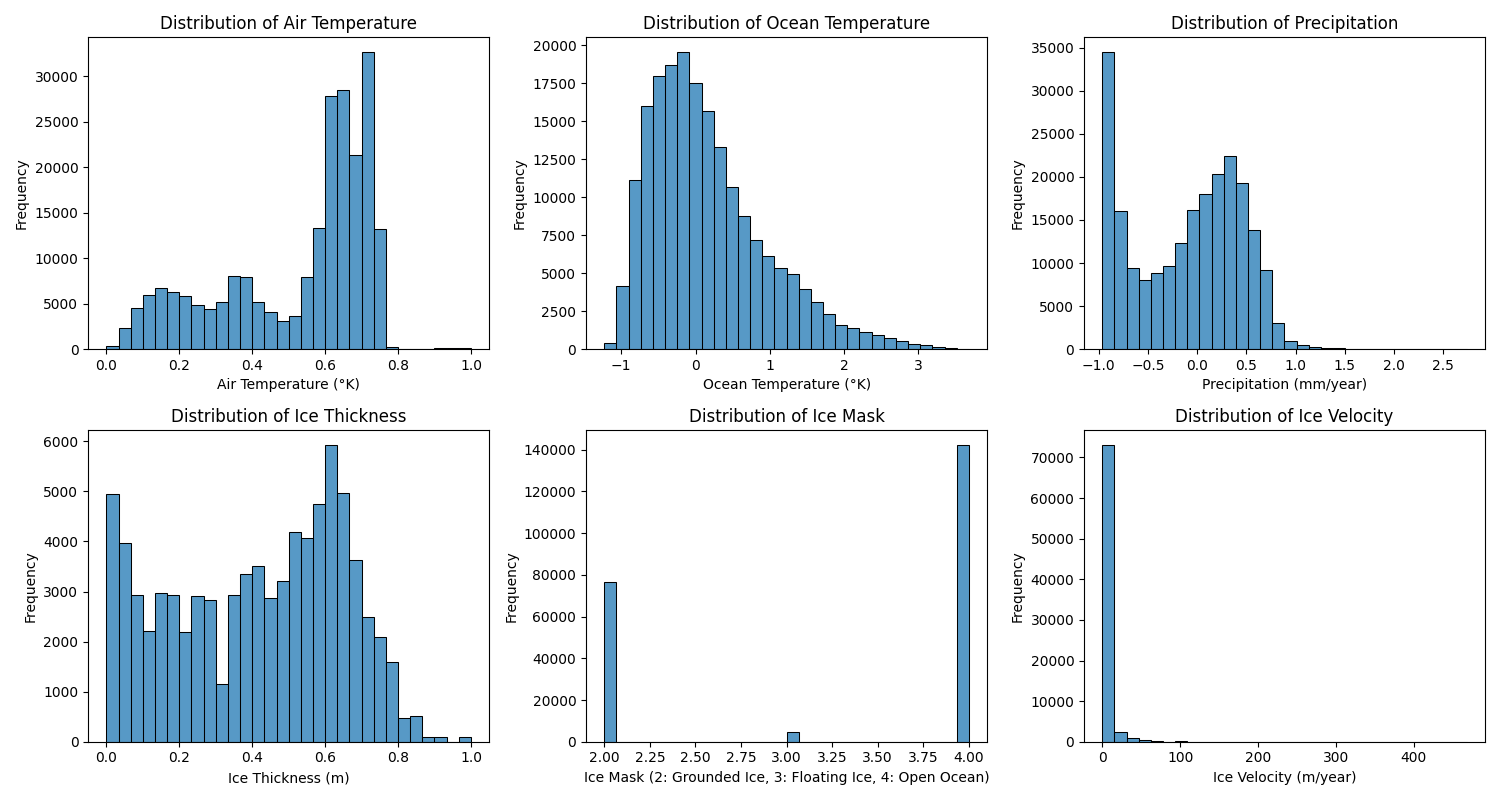
\includegraphics[width=1.2\textwidth]{images/distributions.png}%
    }
  \caption{Histograms Displaying Distributions of Inputs and Outputs}
  \label{fig:distributions}
\end{figure}

The \texttt{air\_temperature} variable shows a mostly unimodal distribution around the mean of 255° K. This distribution is not symmetric, and shows a negative skew with some smaller peaks at 245° K and 227° K respectively.

\texttt{ocean\_temperature} shows a highly unimodal distribution around the mean of 273° K, with no other smaller peaks. This too is slightly asymmetric, but instead with a positive skew.

The final input forcing, \texttt{precipitation}, shows a somewhat bimodal distribution with a large peak at 0mm/year and a smaller peak at 850mm/year. As Antarctica is a desert the high concentration of low precipitation values is to be expected, particularly at lower latitudes \cite{Nicola2023}.

The distribution of \texttt{ice\_thickness} is a less pronounced bimodal distribution with peaks at 0m and 2900m respectively. It should be noted that as described in \Cref{S:IDC}, this distribution excludes values of ocean cells, which would otherwise significantly increase the count of 0m values.

Analysis of \texttt{ice\_mask} is limited due to the discrete nature of this variable. However, it can be noted that most datapoints hold either a value of 2 \textit{(representing grounded ice)} or 4 \textit{(representing open ocean cells)}.

Finally, the distribution of \texttt{ice\_velocity} shows a unimodal distribution with a peak close to 0m/year. There is a positive skew, with some datapoints reaching several thousands of meters a year. This is to be expected, as most of the antarctic ice is either stationary or moving at an extremely slow velocity. This is with the notable exception of certain ice shelves and glaciers that move at comparatively rapid rate \cite{Mouginot2019}.

\subsection{Outliers}\label{SS:outliers}

Next considered was the distribution of outliers for each value, as this provides an opportunity to identify any irregularities or faulty datapoints in the dataset. This can be seen in \Cref{fig:boxplots}.

\begin{figure}[H]
  \centering
  \adjustbox{center}{%
    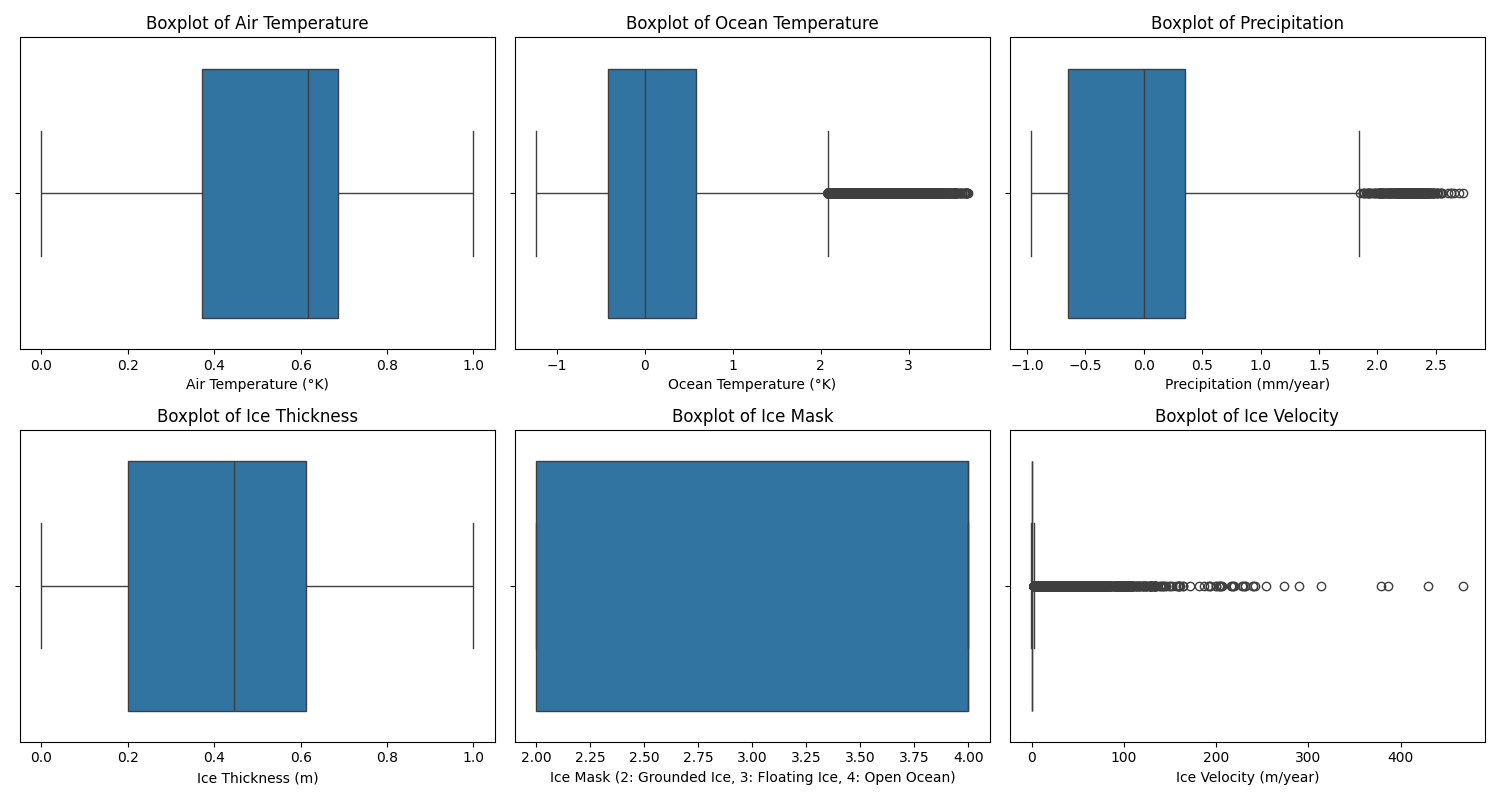
\includegraphics[width=1.2\textwidth]{images/boxplots.png}%
    }
  \caption{Box Plots Detailing Outliers in Each Variable}
  \label{fig:boxplots}
\end{figure}

Half of these variables show no outliers, specifically \texttt{air\_temperature}, \texttt{ice\_thickness}, and \texttt{ice\_mask}. However, all remaining variables display varying distributions of outliers. The \texttt{ocean\_temperature} and \texttt{precipitation} variables both hold significant counts of outlying data points beyond each box plot's maximum \textit{(note the distinction between the maximum of the value, and the maximum of the box plot)}. This indicates these features have highly skewed and leptokurtic distributions that are not fully captured by the extension of each feature's interquartile range.

Finally, the distribution of \texttt{ice\_velocity} outliers appears to contain almost the entire range of the variable. This is likely caused by the extreme skew of this feature, and not representative of truly outlying or incorrect values.

\subsection{Temporal Trends}\label{SS:temporal_trends}

Next considered was the temporal trends of each feature across the 86 years covered in the dataset. The yearly average of each feature was plotted, as can be seen in \Cref{fig:linecharts}.

\begin{figure}[H]
  \centering
  \adjustbox{center}{%
    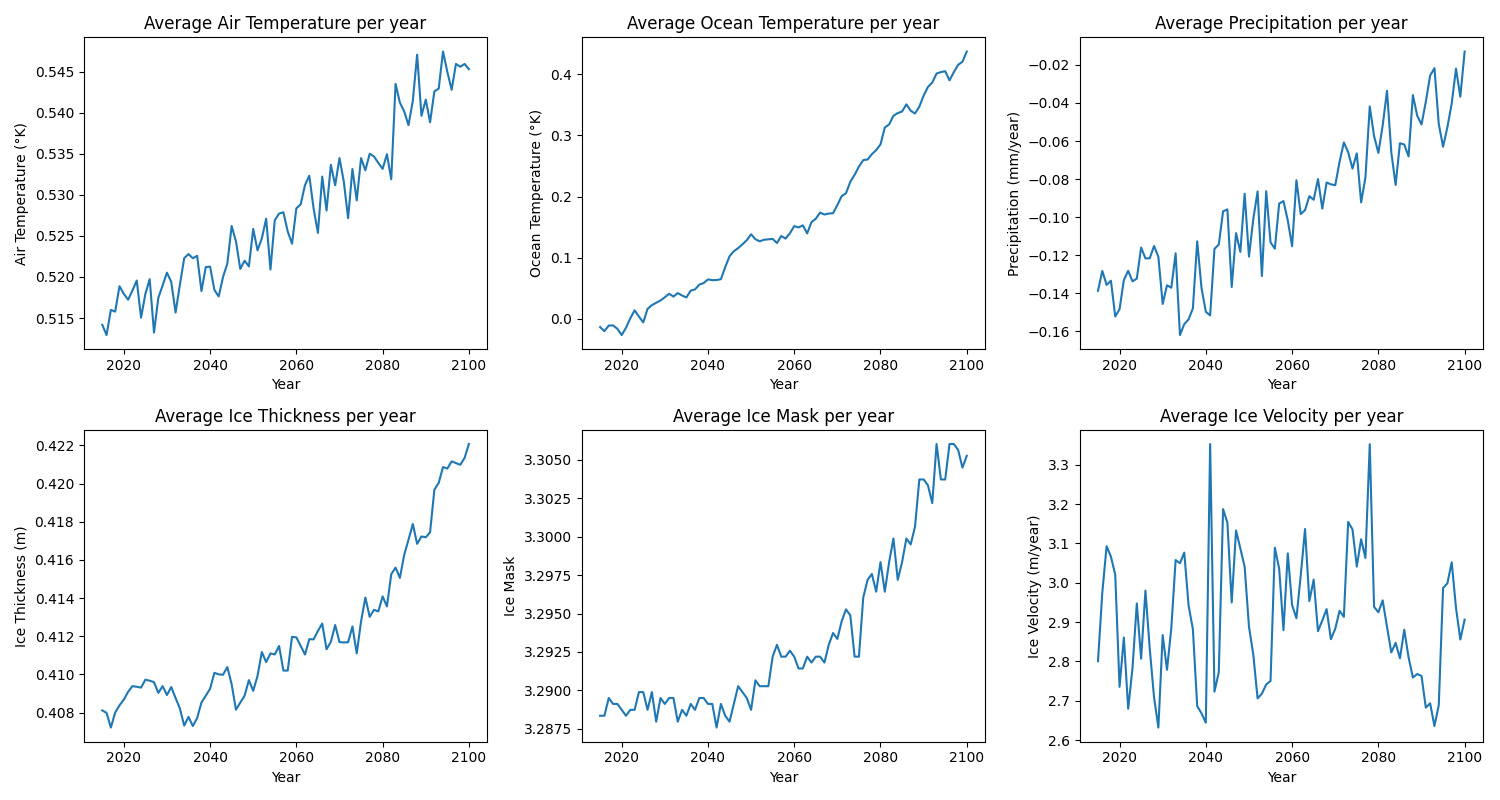
\includegraphics[width=1.2\textwidth]{images/line_charts.png}%
    }
  \caption{Line Charts Displaying Temporal Trends of Inputs and Outputs}
  \label{fig:linecharts}
\end{figure}

With \texttt{ice\_velocity} as the only exception, all charts display a similar positive trend, albeit with slight differences in each feature's variability. This is indicative of a possible correlation between these values, which is ideal for predictive modelling. The \texttt{ice\_velocity} feature shows a much different analysis, with no significant positive or negative trend over time while showing a significantly higher variability relative to other features. This may be due to the particularly skewed distribution causing individual cell variations to have a greater impact on the feature average.

\subsection{Spatial Analysis}\label{SS:spatial_analysis}

Finally, the spatial distribution of each variable was analysed through the use of averaged heatmaps. These display the spatial variance of each feature, and highlight positions with concentrations of particularly high or low values in terms of each feature as can be seen in \Cref{fig:heatmaps}. It should be noted that the heatmaps provided for the \texttt{ice\_thickness} and \texttt{ice\_velocity} variables again have all ocean tiles removed, as detailed in \Cref{S:IDC}.
\begin{figure}[H]
  \centering
  \adjustbox{center}{%
    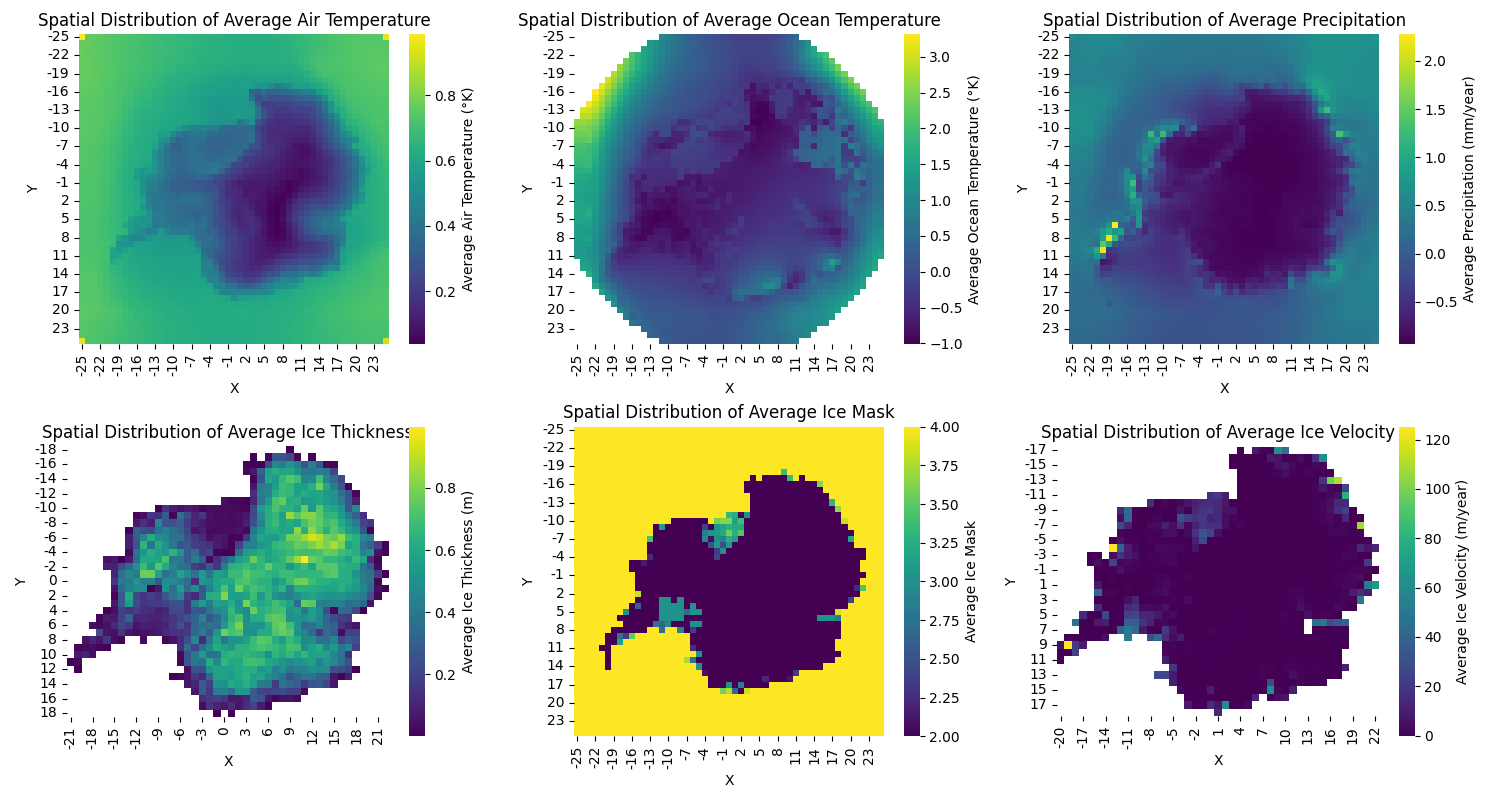
\includegraphics[width=1.2\textwidth]{images/heatmaps.png}%
    }
  \caption{Spatial Heatmaps Displaying Distributions of Inputs and Outputs}
  \label{fig:heatmaps}
\end{figure}

Despite the \texttt{air\_temperature} and \texttt{precipitation} values not encoding land cells directly, the landmass of Antarctica can be clearly identified in both distributions due to the sudden change in values. This could mean these features are more closely correlated with the presence of land. This is supported by the visible similarities to the heatmap of \texttt{ice\_thickness} and \texttt{ice\_mask} values, which directly map the presence of ice and land respectively.

As expected, both \texttt{air\_temperature} and \texttt{ocean\_temperature} display a trend of increasing temperatures as the distance from the south pole increases. 

The \texttt{precipitation} and \texttt{ice\_velocity} variables both show a sharp increase in respective values around the coastlines, each with very low values across the interior of the continent. This sudden increase is particularly prominent across the eastern edge of the Antarctic Peninsula. In terms of precipitation, this is expected as the sudden change of atmospheric conditions following coastlines often causes more rainfall \cite{Bromwich1990}. Similarly, the coastlines are where many ice shelves deposit ice into the ocean, so higher readings of \texttt{ice\_velocity} are to be expected \cite{Mouginot2019}.

\section{Correlation Analysis}\label{SS:correlation_analysis}
To further analyse the correlations between each variable, a correlation matrix was produced. The insight this provides is twofold; 

\begin{enumerate}
    \item  The correlations between input features can be useful for identifying redundancy and therefore possible areas for dimensionality reduction, improving model training times with minimal cost to predictive performance \cite{Rovira2022}.
    \item The correlative values between input features and target outputs provide initial analysis for the predictive capabilities of each input feature \textit{(i.e. the strength at which each input aides in prediction)} \cite{Hall2000}.
\end{enumerate}


\begin{figure}[H]
  \centering
  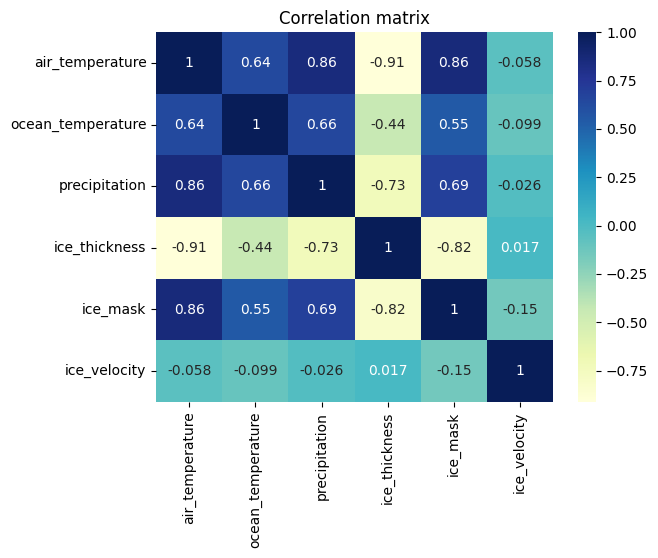
\includegraphics[width=1\textwidth]{images/correlations.png}
  \caption{Correlation Heatmap of Variables}
  \label{fig:correlations}
\end{figure}
The magnitude of the correlation signifies how closely each pairing is matched, with the sign denoting whether this is a positive or negative relationship \textit{(positive here meaning one variable increases with another)}.

The features \texttt{air\_temperature} and \texttt{precipitation}  show a high correlation with a value of 0.86. This relationship is further supported with evidence in the form of similar heatmaps seen in \Cref{fig:heatmaps} and similar line charts seen in \Cref{fig:linecharts}. The high magnitude and positive value of this correlation indicates a highly colinear relationship. This relationship may be explained by the tendency for warmer temperatures to lead to higher rates of evaporation, and thus precipitation  \cite{Nicola2023}.  As would be predicted by atmospheric heat exchange, \texttt{ocean\_temperature} and \texttt{air\_temperature} also display a positive correlation \cite{Bromwich1990}. These relationships \textit{(those of \texttt{ocean\_temperature} → \texttt{air\_temperature} and \texttt{air\_temperature} → \texttt{precipitation})} are transitive, with the \texttt{precipitation} → \texttt{ocean\_temperature} showing a similarly high correlation of 0.66.

The highest magnitude correlation is between \texttt{ice\_thickness} and \texttt{air\_temperature} with a value of -0.91. This value indicates these variables are highly correlated , but with a negative relationship. The transitive relationships mentioned previously also hold true here, with \texttt{ice\_thickness} correlating to \texttt{ocean\_temperature} and \texttt{precipitation} with values of -0.44 and -0.77 respectively. This is promising as it indicates this target output may be relatively simple to accurately model from the input features alone \cite{Hall2000}.

The \texttt{ice\_velocity} feature holds the lowest correlation values across all other variables, with an average correlation of -0.07.  This also indicates this target output may be harder to predict than other values.

\section{Preprocessing}

With this initial analysis in mind, several steps were taken for further preprocessing. This included changes to encoding, scaling procedures, and filling of any remaining empty values. 

\subsection{Filling Values}

The removal of values in \Cref{S:IDC} allowed for more detailed analysis of feature distributions in \Cref{S:UVA}, but this is not viable for further modelling due to the inherent need for numerical values in many architectures. As such, the remaining empty values in the \texttt{ice\_thickness} and \texttt{ice\_velocity} variables were filled with a placeholder value of 0 to signify a lack of ice. 

\subsection{Positional Encoding}

The \texttt{x\_coordinate} and \texttt{y\_coordinate} values were altered from the original scale, which ranged 6,080,000m in intervals of 121,600m \textit{(centered around the south pole at (0,0))}. Instead, these intervals were transformed into cell indexes ranging from -25 to 25 for each coordinate, still centered at (0,0). While not directly useful for modelling, this representation is simpler for cell indexing and feature engineering.

\subsection{Scaling}

As this project aims to incorporate a variety of predictive models, special note should be taken for scaling so as to avoid preemptively harming the predictive accuracy of any models produced \cite{Ahsan2021}. 

Several variables were not altered, including the positional constants \textit{(\texttt{x\_coordinate} and \texttt{y\_coordinate})}, the derived \texttt{year} value, and \texttt{ice\_mask}. No transform steps were applied on these, as each variable was already suitably encoded.

Robust scaling was applied to \texttt{ocean\_temperature}, \texttt{precipitation}, and \texttt{ice\_velocity}, as these variables were identified as containing highly skewed distributions with many outliers \textit{(See \Cref{SS:outliers})}. All other variables were scaled with a simple Min-Max scaler.


\section{Feature Engineering}\label{S:feature_engineering}

Feature engineering provides an opportunity to improve predictive accuracy by deriving additional features from the original dataset. This was managed carefully, as increasing the dimensionality of the input data can significantly slow model training times. Several iterations of creating and analyzing features were completed, but few of these provided novel correlative values that may improve model performance. These include:

\begin{enumerate}
    \item \textbf{\texttt{dtp} \textit{(Distance to Pole)}} - A measure of each cell's euclidean distance to the central grid point \textit{(0,0)}. This provides a high correlation value with the \texttt{ice\_mask} target.
    \item \textbf{Rolling Standard Deviations (×2)} - A rolling kernel applied to the grid calculating the standard deviation for both \texttt{precipitation} and \texttt{air\_temperature} values across the 8 surrounding neighbor cells. These were the only measures that provided improved correlation measures against \texttt{ice\_velocity}.
    \item \textbf{\texttt{temp\_diff} \textit{(Temperature Difference)}} - A measure of the temperature \textit{(K°)} difference between \texttt{air\_temperature} and \texttt{ocean\_temperature} values. This provided high magnitude correlation values for both \texttt{ice\_thickness} and \texttt{ice\_mask}.
    \item \textbf{\texttt{log\_air\_temperature} \textit{(Log Transform)}} - A simple log transform applied to the \texttt{air\_temperature}. This transform was applied to all input features, but only \texttt{air\_temperature} provided beneficial correlation values, particularly with regard to \texttt{ice\_thickness} and \texttt{ice\_mask}. 
\end{enumerate}
The correlations with respect to the target outputs can be viewed in \Cref{fig:created_feature_correlations}.
\begin{figure}[H]
  \centering
  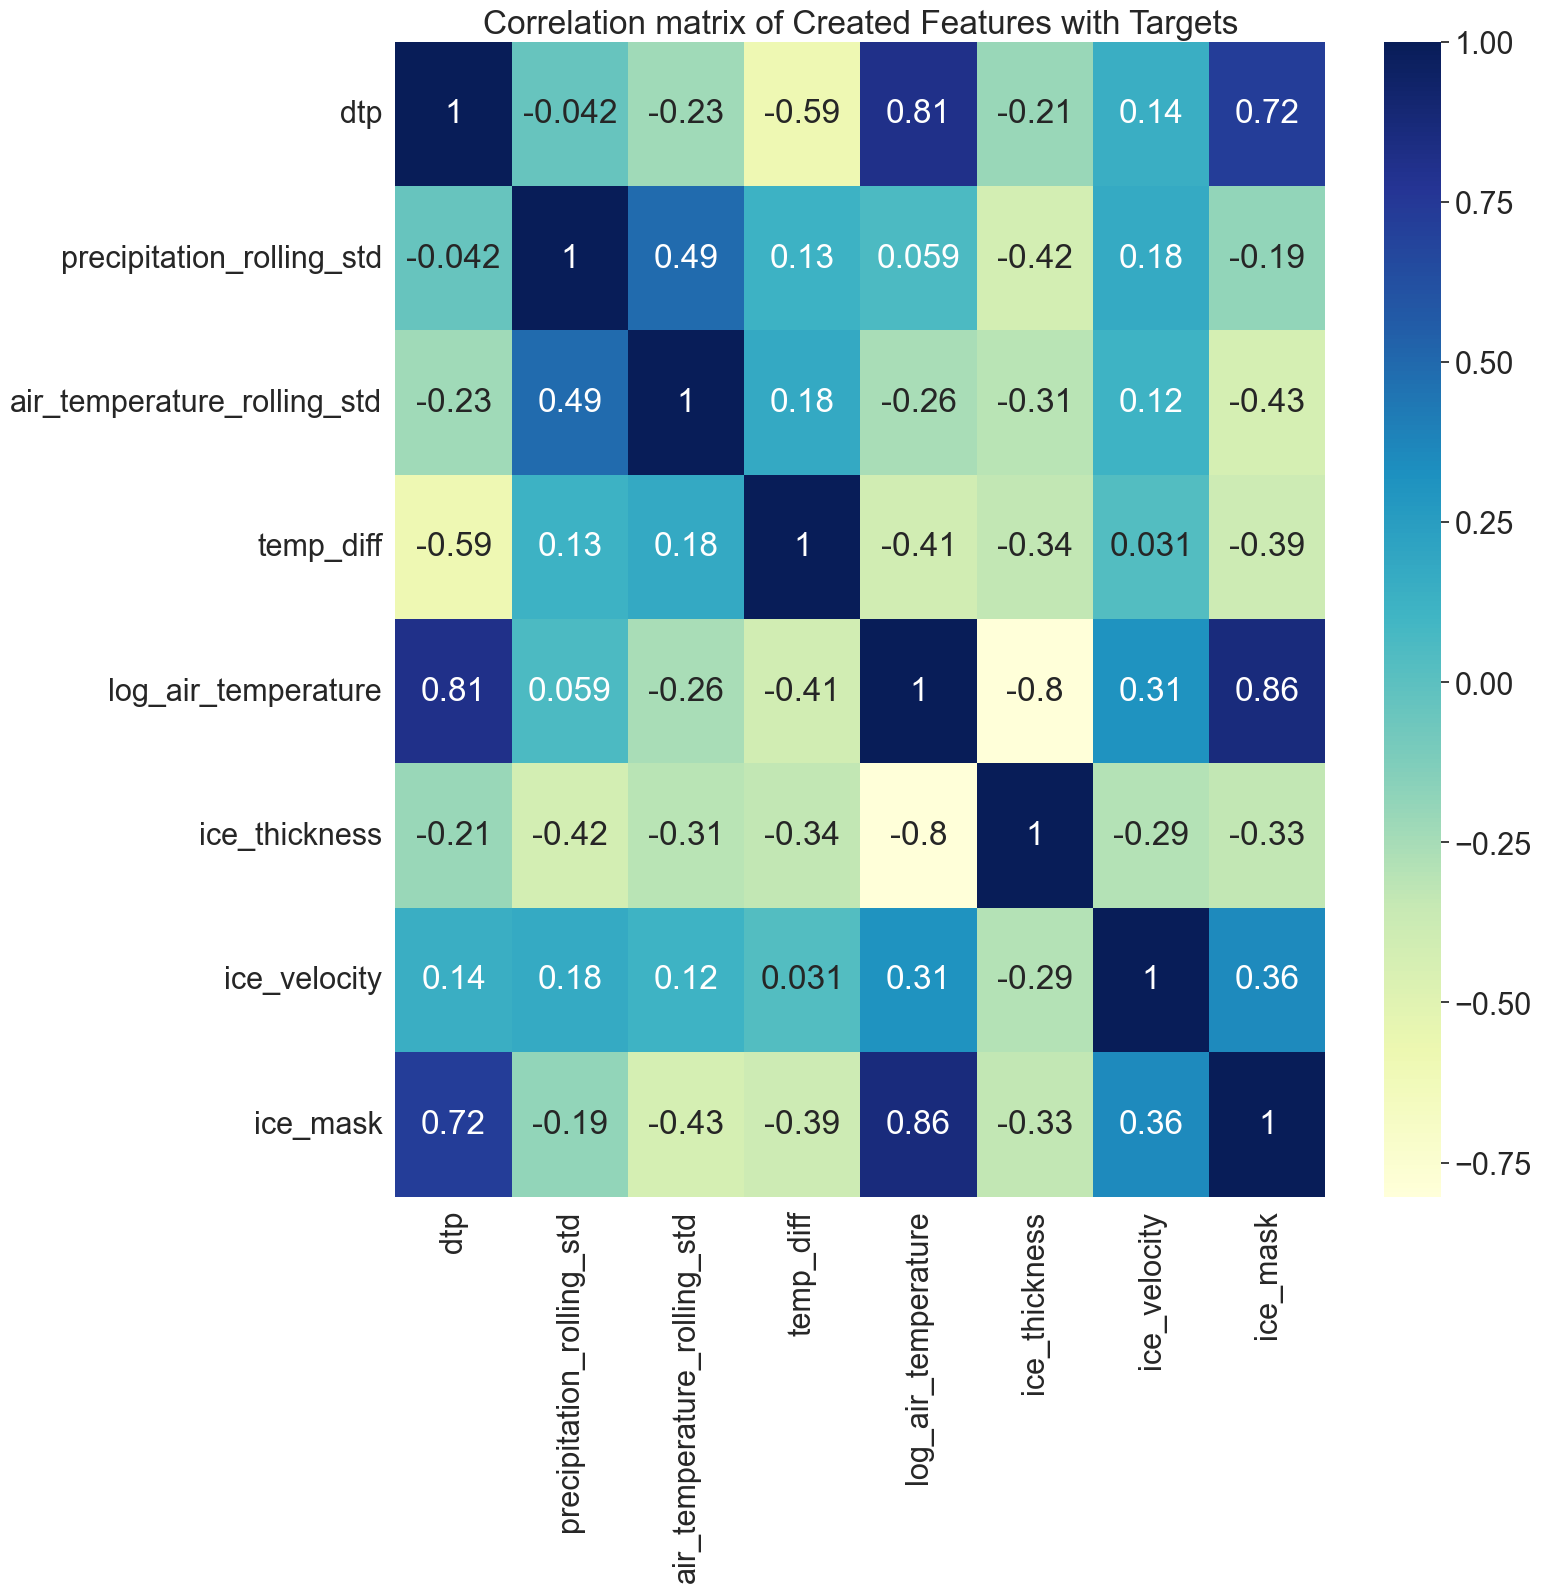
\includegraphics[width=0.75\textwidth]{images/feature_creation_correlations.png}
  \caption{Correlation Heatmap of Created Features and Targets}
  \label{fig:created_feature_correlations}
\end{figure}
\begin{figure}[H]
  \centering
  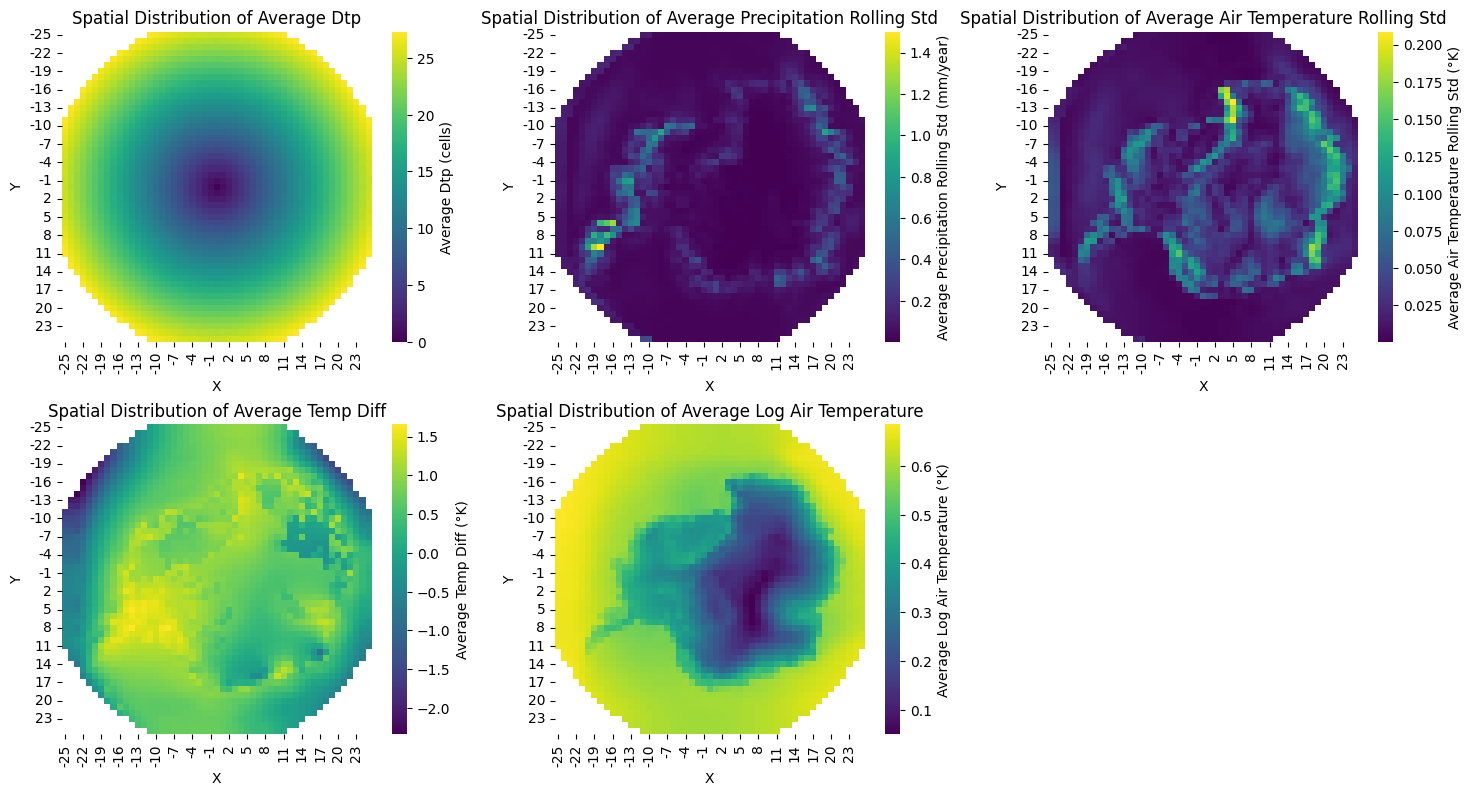
\includegraphics[width=1\textwidth]{images/feature_creation_heatmaps.png}
  \caption{Spatial Heatmaps of Created Features}
  \label{fig:created_feature_heatmaps}
\end{figure}

These heatmaps \textit{(see \ref{fig:created_feature_heatmaps})} provide an interesting visual analysis of the created features. Particularly of note is the two rolling standard deviation measures, as these appear to form a pattern tracing the coastline of the ice shelves. This may explain why these measures have higher correlative values with the \texttt{ice\_velocity}, as this variable has a similar spatial distribution.

With feature engineering complete, this leaves the initial EDA completed and the dataset prepared for further development and modelling.